As already specified, CMS maintains a huge amount of data, O(50PB), organized 
in datasets, which share common properties and users tend to analyze as a whole. 
Datasets are further subdivided into data blocks consisting of one or more files. These 
subdivisions facilitate the handling of the datasets.

A convenient set of tools exists to move data around but there is no intelligent tool to produce and
distribute copies of popular data or automatically remove less popular data. At present the various 
physics groups each have a data manager who is responsible for disk management. Usually this involves 
the management of about three Tier-2 computing sites and about a thousand 
datasets (mostly Monte Carlo simulation). Placement of new data is relatively straight forward but the 
deletion of older sets can be quite complicated and requires significant amount of time.

At MIT, we have tried to tackle this problem by considering a small subset of the CMS computing system, 
i.e. the two sites sub-system \{T2\_US\_MIT,T3\_US\_MIT\}. In this sub-system we have the following:

\begin{itemize}
	\item all datasets relevant for MIT analyses are stored on the Tier-2;
	\item all data analysis jobs are run on Tier-3 machines;
	\item the available disk space of the Tier-3 is not enough to store all datasets necessary for 
	the completion of all the analyses.
	\item users typically re-run a given analysis workflow multiple times on the same group of datasets in 
	a relatively short timescale.
\end{itemize}
We have designed and implemented an automated service, the \textbf{MIT HEP Dynamic Data (MITHDD)}, that 
caches the datasets on Tier-3, using the Tier-2 as a source pool. 

MITHDD is divided into two subservices: \textbf{SmartCache}, which is responsible for transferring 
datasets from Tier-2 to Tier-3, and \textbf{Cinderella}, which is responsible for deletions on Tier-3.

The source code of MITHDD follows the same structure and is currently available on \textsc{GitHub} at 
\href{https://github.com/cpausmit/DynamicData}{\textcolor{Mahogany}{this link}}. The software is licensed
under \href{http://opensource.org/licenses/MIT}{\textcolor{Mahogany}{these terms}}.

\subsection{SmartCache}\label{subsec:smartcache}
The scope of SmartCache is to create and handle transfer requests needed to ensure that 
user jobs, running on Tier-3, can analyze datasets stored only on the Tier-2. Datasets are organized into 
files, which are mapped in the SmartCache \textsc{MySQL} database. These files are the fundamental blocks 
managed by SmartCache. A system daemon interfaces with the file database, and it periodically 
performs the following operations:

\begin{enumerate}
	\item collects dataset requests, if any, and checks which files are not stored on Tier-3;
	\item creates transfers requests for all files that need to be transferred on Tier-3;
	\item keeps track of pending transfers until they are completed;
	\item saves relevant information for each transfer (status, speed, ecc...);
	\item updates the file database.
\end{enumerate}

The daemon exploits the Tier-3 batch system to submit jobs for file transfers. The transfer technology 
is based on LCG Data Management Client Tools, supported by the OSG consortium~\cite{OSG1,OSG2}. The use of 
the batch system for downloads allows concurrent multiple file transfers, limited only by the number slots 
allocated for this particular service. This model is particularly interesting as it can be scaled with minimal 
effort, since the allocation and management of the batch system slots is performed with standard cluster 
tools (in the case of our site \textsc{HTCondor}).

\subsubsection{SmartCache Monitoring}

We have also designed and implemented a system that periodically checks the status of SmartCache, analyzes it
and produces plots in order to track the performance of our caching system.

The monitoring tool computes and plots the following distributions:

\begin{itemize}
	\item \textbf{SmartCache transfer rate}, which shows the cumulative transfer speed for the caching jobs at
	any given time;
	\item \textbf{SmartCache transfer failures}, i.e. the rate of failed transfers as a function of time;
	\item \textbf{Lag time}, which shows the time lapse between the file download request and the start of the file transfer;
	\item \textbf{Speed}, i.e. the file transfer rate (not cumulative).
\end{itemize}

These distributions are computed for five different time periods - last hour, last day, last week, last month, all times - 
and are uploaded to the web and available at 
\href{http://t3serv001.mit.edu/~paus/plots/}{\textcolor{Mahogany}{this link}}.

As an example of the monitoring output, we report in Figure~\ref{fig:SmartCache} the summary plots for the month of
August 2014. 

\begin{figure}[htbp]
 \centering
 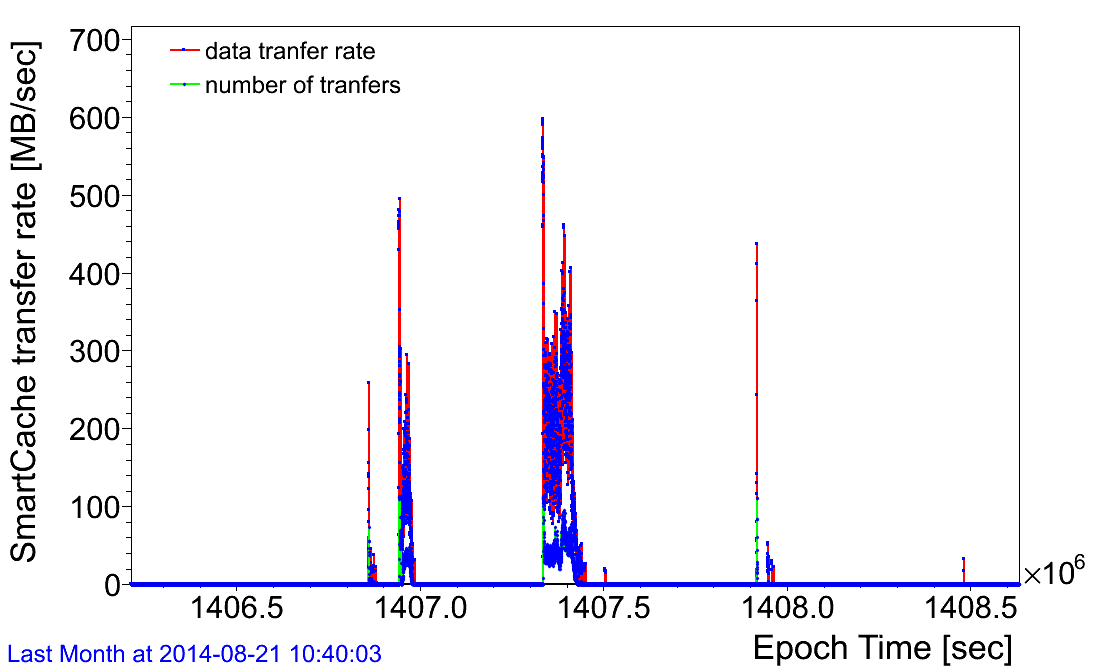
\includegraphics[angle=0,width=0.49\textwidth]{plots/transferRateLastMonth.png}
 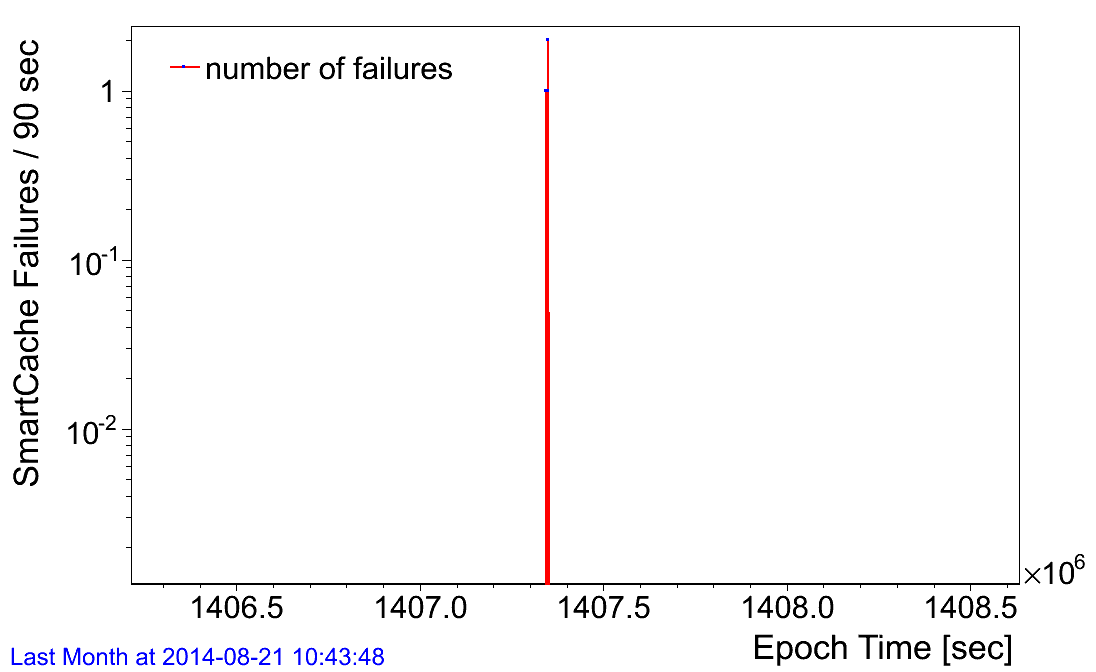
\includegraphics[angle=0,width=0.49\textwidth]{plots/failuresLastMonth.png}
 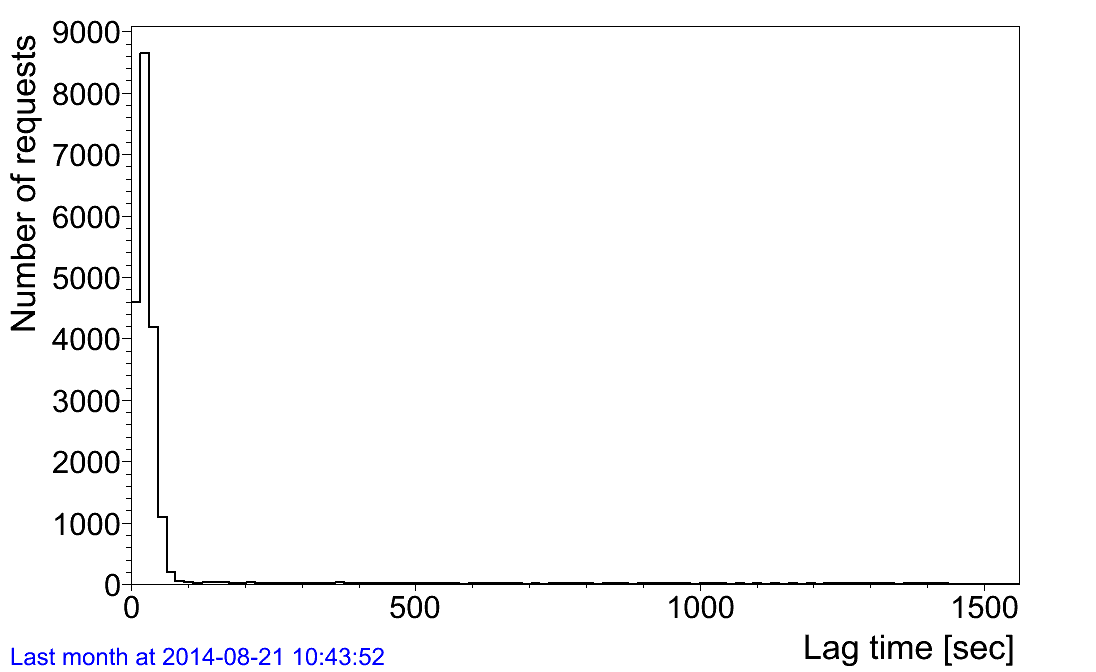
\includegraphics[angle=0,width=0.49\textwidth]{plots/lagTimeLastMonth.png}
 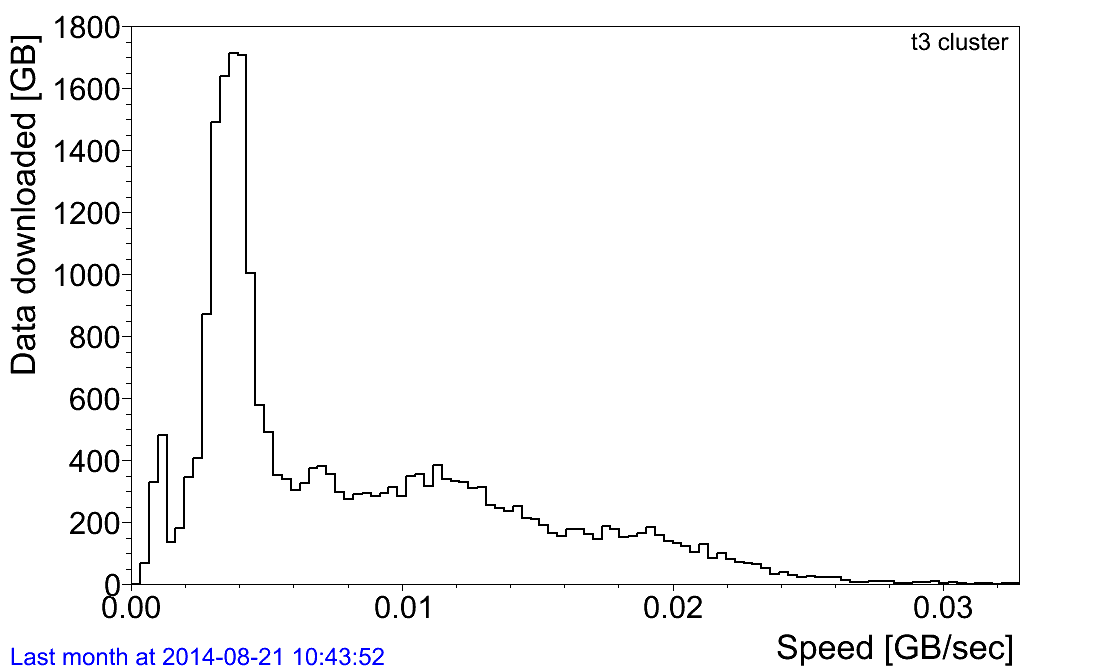
\includegraphics[angle=0,width=0.49\textwidth]{plots/downloadSpeedLastMonth.png}
 \caption{SmartCache monitoring plots for the month of August 2014. In the figures, from top row to bottom row, left to right,
 SmartCache transfer rate, SmartCache transfer failures, Lag time and Speed.}
 \label{fig:SmartCache}
\end{figure}

For of our site, it is interesting to look at Figure~\ref{fig:SmartCache} top-left. First of all it 
shows that we can cache datasets at a total speed of about 5 Gb/s. In addition, we could possibly improve this by
adding more machines to our cacher pool:
at T3\_US\_MIT there are currently 33 machines dedicated to transfers, each carrying an average of three slots, 
thus up to about 100 transfers can happen. Even considering the bandwidth limitation of each machine, we would expect
to be able to saturate our uplink speed, i.e. 8 Gb/s. Nevertheless, the
rate plot shows that the maximum caching speed saturates at 60\% of the total available bandwidth.
Thus, we are limited by some non-network related factors (likely the disk writing speed on TNs).


\subsection{Cinderella}\label{subsec:cinderella}
The design of Cinderella follows the requirements of an automatic cache release process needed for the 
CMS computing. This cache release process is supposed to optimize the usage of all 
available disk storage and relieve the data managers of a large fraction of their work by:

\begin{enumerate}
	\item keeping all storage filled to a high and safe level;
	\item always allow new data to be received at any site;
	\item remove the least valuable data from the storage when the storage fills over a given level.
\end{enumerate}

In order to perform a cache release, the system is periodically reviewed to ensure there is free space 
for transfers at the site. The condition for the cache release is given by:

\begin{itemize}
	\item usedSpace / availableSpace $>$ 92\% (number can be adjusted);
\end{itemize}

When the cache release algorithm is triggered, enough datasets to restore the target free space are identified
for deletion in order to fulfill the following condition:

\begin{itemize}
	\item usedSpace / availableSpace $<$ 87\% (number can be adjusted);
\end{itemize}

To select datasets for deletion we algorithmically rank all datasets. We select datasets with the lowest priority
by adding the space they occupy until we have enough space to meet the above condition. The selected datasets are 
then removed from storage. The ranking algorithm evaluates the usefulness of the data. For our site, the ranking 
algorithm uses only the time of latest access, such that the lowest priority datasets were accessed longest ago. 

Cinderella implements the algorithm described above. The core parts of the software are
a \textsc{MySQL} database, which stores the list of datasets and relevant information needed to generate the ranking
and perform the cache release, and a daemon that periodically checks if the release trigger condition is met.
In case of a triggered release, the Cinderella daemon issues the deletion command and updates the dataset database.

The Cinderella service also takes periodic snapshots of the dataset database, and uploads them online at 
\href{http://t3serv001.mit.edu/~cmsprod/dynamicdata/cinderella.html}{\textcolor{Mahogany}{this webpage}}.
The snapshots show a ranked list of datasets in our database according to the algorithm used for the
cache release. For each dataset, the number of accesses, number of downloads, caching status (which 
determines if that dataset is present on the Tier-3 cache), last access time and size are listed.
In the current color scheme, blue denotes datasets that were at some point cached but have been deleted and
are not currently stored in cache, red shows the list of datasets that will be deleted in case the cache release
condition is met, and black shows the remaining datasets.

During 6 months of operations, Cinderella has been responsible for deletions that amount to a total of 0.1 PB
of disk space, equivalent to 1/3 of the entire Tier-3 storage capabilities. Equivalently, the system has 
triggered a cache release about ten times.







